\documentclass[border=20pt]{standalone}
\usepackage{amsfonts}
\usepackage{amsmath}
\usepackage{amssymb}
\usepackage{tabularx}
\usepackage{multicol}
\usepackage{multirow}
\usepackage{physics}
\usepackage{siunitx}
\usepackage{bm}
\usepackage{booktabs}
\usepackage{enumitem}
\usepackage{longtable}
\usepackage{array}
\usepackage{bm}
\usepackage{tikz}
\usepackage{pgfplots}
\usepackage[outline]{contour} % glow around text
\usetikzlibrary{calc}
\usetikzlibrary{angles,quotes} % for pic
\usetikzlibrary{arrows.meta}
\usetikzlibrary{patterns}
\tikzset{>=latex} % for LaTeX arrow head
\contourlength{1.35pt}

%Tikz Library
\usetikzlibrary{angles, quotes, intersections}

		
		

\colorlet{xcol}{blue!70!black}
\colorlet{vcol}{green!60!black}
\colorlet{myred}{red!65!black}
\colorlet{mydarkred}{red!40!black}
\colorlet{mypurple}{blue!60!red!80}
\colorlet{mydarkgreen}{green!20!black}
\colorlet{acol}{red!50!blue!80!black!80}
\tikzstyle{rvec}=[->,xcol,very thick,line cap=round]
\tikzstyle{vvec}=[->,vcol,very thick,line cap=round]
\tikzstyle{myarr}=[{Latex[length=3,width=3]}-,xcol]
\tikzstyle{myarr2}=[{Latex[length=2,width=2.5]}-{Latex[length=2,width=2.5]}]
\tikzstyle{force}=[->,myred,very thick,line cap=round]
\tikzstyle{Fproj}=[force,myred!40]
\tikzstyle{CM}=[mydarkred,fill=red!80!black!80]


\tikzstyle{mass}=[line width=0.6,draw=red!30!black, %rounded corners=1,
                  top color=mydarkred!30,bottom color=mydarkred!10,shading angle=30]

\tikzstyle{mass2}=[line width=0.4,draw=black, %rounded corners=1,
                  top color=black!40,bottom color=black!40]
                  
\tikzstyle{dark mass}=[line width=0.3,red!30!black, %rounded corners=1,
                       top color=mydarkred!40,bottom color=mydarkred!60,shading angle=30]
\tikzstyle{ground}=[preaction={fill,top color=black!10,bottom color=black!5,shading angle=20},
                    fill,pattern=north east lines,draw=none,minimum width=0.3,minimum height=0.6]
\tikzstyle{metal}=[fill,top color=black!40,bottom color=black!20,shading angle=10]
\tikzstyle{pulcol}=[draw=blue!30!black,%fill=blue!40!black!10
                    top color=blue!40!black!20,bottom color=blue!40!black!10,shading angle=20]
\tikzstyle{rope}=[brown!70!black,very thick,line cap=round]
\def\rope#1{ \draw[black,line width=1.5] #1; \draw[rope] #1; }
\tikzstyle{mount}=[blue!20!black,fill,top color=blue!20!black!70,bottom color=blue!20!black!40,shading angle=10]

\def\r{0.05} % pulley small radius
\tikzset{
  pics/Tin/.style={
    code={
      \def\R{0.12}
      \draw[pic actions,line width=0.6,#1,fill=white] % ,thick
        (0,0) circle (\R) (-135:.75*\R) -- (45:.75*\R) (-45:.75*\R) -- (135:.75*\R);
  }},
  pics/Tout/.style={
    code={
      \def\R{0.12}
      \draw[pic actions,line width=0.6,#1,fill=white] (0,0) circle (\R);
      \fill[pic actions,#1] (0,0) circle (0.3*\R);
  }},
  pics/rotarr/.style={
    code={
      \draw[white,very thick] ({#1*cos(200)},0) arc(-200:30:{#1} and {#1/2}) --++ (125:0.1);
      \draw[->,mydarkgreen] ({#1*cos(200)},0) coordinate (W1) arc(-200:20:{#1} and {#1/2}) node[midway] (W2) {} --++ (125:0.1) coordinate (W3);
  }},
  pics/pulley/.style={
    code={
      \draw[pulcol,line width=0.6] (0,0) circle (#1);
      \draw[pulcol,thick] (0,0) circle (\r);
  }},
  pics/mount/.style args={#1:#2}{ % angle, length
    code={
      \draw [mount] (0,0)++(#1-90:0.9*\r) arc (#1-90:#1-270:0.9*\r) --++ (#1:#2) --++ (#1-90:1.8*\r) -- cycle;
    }
  },
  pics/Tin/.default=mypurple,
  pics/Tout/.default=mypurple,
  pics/rotarr/.default=0.4,
  pics/pulley/.default=0.3,
}


\newcommand\rightAngle[4]{
  \pgfmathanglebetweenpoints{\pgfpointanchor{#2}{center}}{\pgfpointanchor{#3}{center}}
  \coordinate (tmpRA) at ($(#2)+(\pgfmathresult+45:#4)$);
  \draw[white,line width=0.7] ($(#2)!(tmpRA)!(#1)$) -- (tmpRA) -- ($(#2)!(tmpRA)!(#3)$);
  \draw[xcol!30!black] ($(#2)!(tmpRA)!(#1)$) -- (tmpRA) -- ($(#2)!(tmpRA)!(#3)$);
}


\setlength\parindent{0pt}

\begin{document}

% MOMENT OF INERTIA - HOLLOW CYLINDER
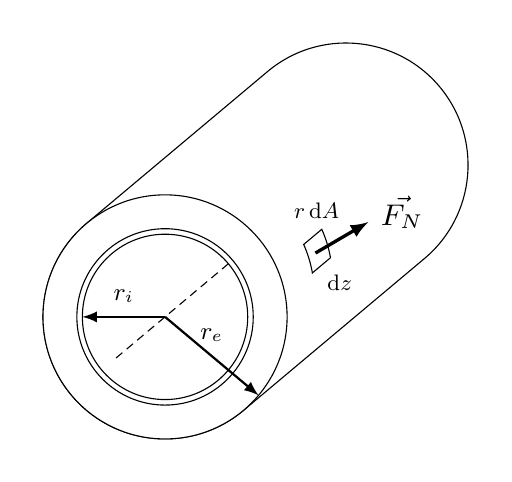
\begin{tikzpicture}
  \Large
  \def\L{3.0} % cylinder length
  \def\R{1.4}
  \def\dr{0.15}
  \def\ang{10}
  \def\angp{40} % perspective
  \def\angdr{14}
  \coordinate (O) at (0,0);
  \coordinate (R) at (\ang:\R);
  \draw[fill=none,
    top color=white,bottom color=white,middle color=white]
    (\angp+90:\R+\dr) --++ (\angp:\L) arc(\angp+90:\angp-90:\R+\dr) --++ (\angp-180:\L) arc(\angp-90:\angp-270:\R+\dr);
  \draw[fill=white,even odd rule]
    circle(\R+\dr);
   \draw[fill=white,even odd rule]
    (O) circle(\R*0.8) circle(\R*0.75);
  %\draw[dashed,thick] (\angp:0.98*\R) -- (\angp-180:1.7*\R);
  \draw[densely dashed] (\angp:\R*0.75) -- (\angp-180:\R*0.6) node[left] {};
  \draw[fill=none]
    (\ang:\R+\dr)++(\angp:0.25*\L) coordinate (DM1)
    arc(\ang:\ang+\angdr:\R+\dr) {}
    --++ (\angp-180:0.1*\L) arc(\ang+\angdr:\ang:\R+\dr) -- cycle;
  \draw[white] (DM1)++(-70:0.08) --++ (\angp-180:0.1*\L)
    node[midway,black,below right=-3,scale=0.9] {\small $\dd{z}$};
  \draw[-,white, thick] (DM1)++(20:0.08) arc(\ang:\ang+\angdr:\R+\dr);
  \node at (35:2.35) [black,scale=0.9] {\small $r\dd{A}$};
  \coordinate (DM2) at (\ang+13:\R+\dr*4.5)++(\angp:0.25*\L);
  \draw[->, black, very thick] (DM2) -- (25:2.85); 
  \node[left=-1,scale=1.2] at (21:3.7) {\small $\vec{F_N}$};
  \draw[->, thick] (O) -- (-40:\R+\dr/1) node[midway, above] {\contour{white}{\small $r_e$}};
  \draw[->, thick] (O) -- (180:\R*0.75) 
  node[midway, above] {\contour{white}{\small $r_i$}};
 
\end{tikzpicture}
\end{document}